\documentclass[11pt,a4paper]{article}
\usepackage[utf8]{inputenc}
\usepackage[spanish]{babel}
\usepackage[margin=2.5cm]{geometry}
\usepackage{graphicx}
\usepackage{hyperref}
\usepackage{xcolor}
\usepackage{enumitem}
\usepackage{array}
\usepackage{booktabs}
\usepackage{tikz}
\usepackage{amssymb}
\usepackage{listings}
\usetikzlibrary{shapes,arrows,positioning,fit,backgrounds}

% Configuración de listings para código
\definecolor{codegreen}{rgb}{0,0.6,0}
\definecolor{codegray}{rgb}{0.5,0.5,0.5}
\definecolor{codepurple}{rgb}{0.58,0,0.82}
\definecolor{backcolour}{rgb}{0.95,0.95,0.92}

\lstset{
    backgroundcolor=\color{backcolour},   
    commentstyle=\color{codegreen},
    keywordstyle=\color{magenta},
    numberstyle=\tiny\color{codegray},
    stringstyle=\color{codepurple},
    basicstyle=\ttfamily\footnotesize,
    breakatwhitespace=false,         
    breaklines=true,                 
    captionpos=b,                    
    keepspaces=true,                 
    numbers=left,                    
    numbersep=5pt,                  
    showspaces=false,                
    showstringspaces=false,
    showtabs=false,                  
    tabsize=2
}

% Configuración de links
\hypersetup{
    colorlinks=true,
    linkcolor=blue,
    urlcolor=blue,
    pdftitle={Reporte Actividad 6 - Digimon API}
}

% Colores personalizados para el diagrama
\definecolor{frontend}{RGB}{79,70,229}
\definecolor{backend}{RGB}{147,51,234}
\definecolor{externalapi}{RGB}{14,165,233}
\definecolor{client}{RGB}{16,185,129}

\begin{document}

% --- PORTADA ---
\begin{titlepage}
    \centering
    \vspace*{1cm}
    {\huge \textbf{Universidad Politécnica de Chiapas}} \\[1.5cm]
    {\large \textbf{Ingeniería en Desarrollo de Software}} \\[0.5cm]
    {\large \textbf{Actividad No. 6: Exposición y Consumo de APIs de Terceros}} \\[2cm]
    
    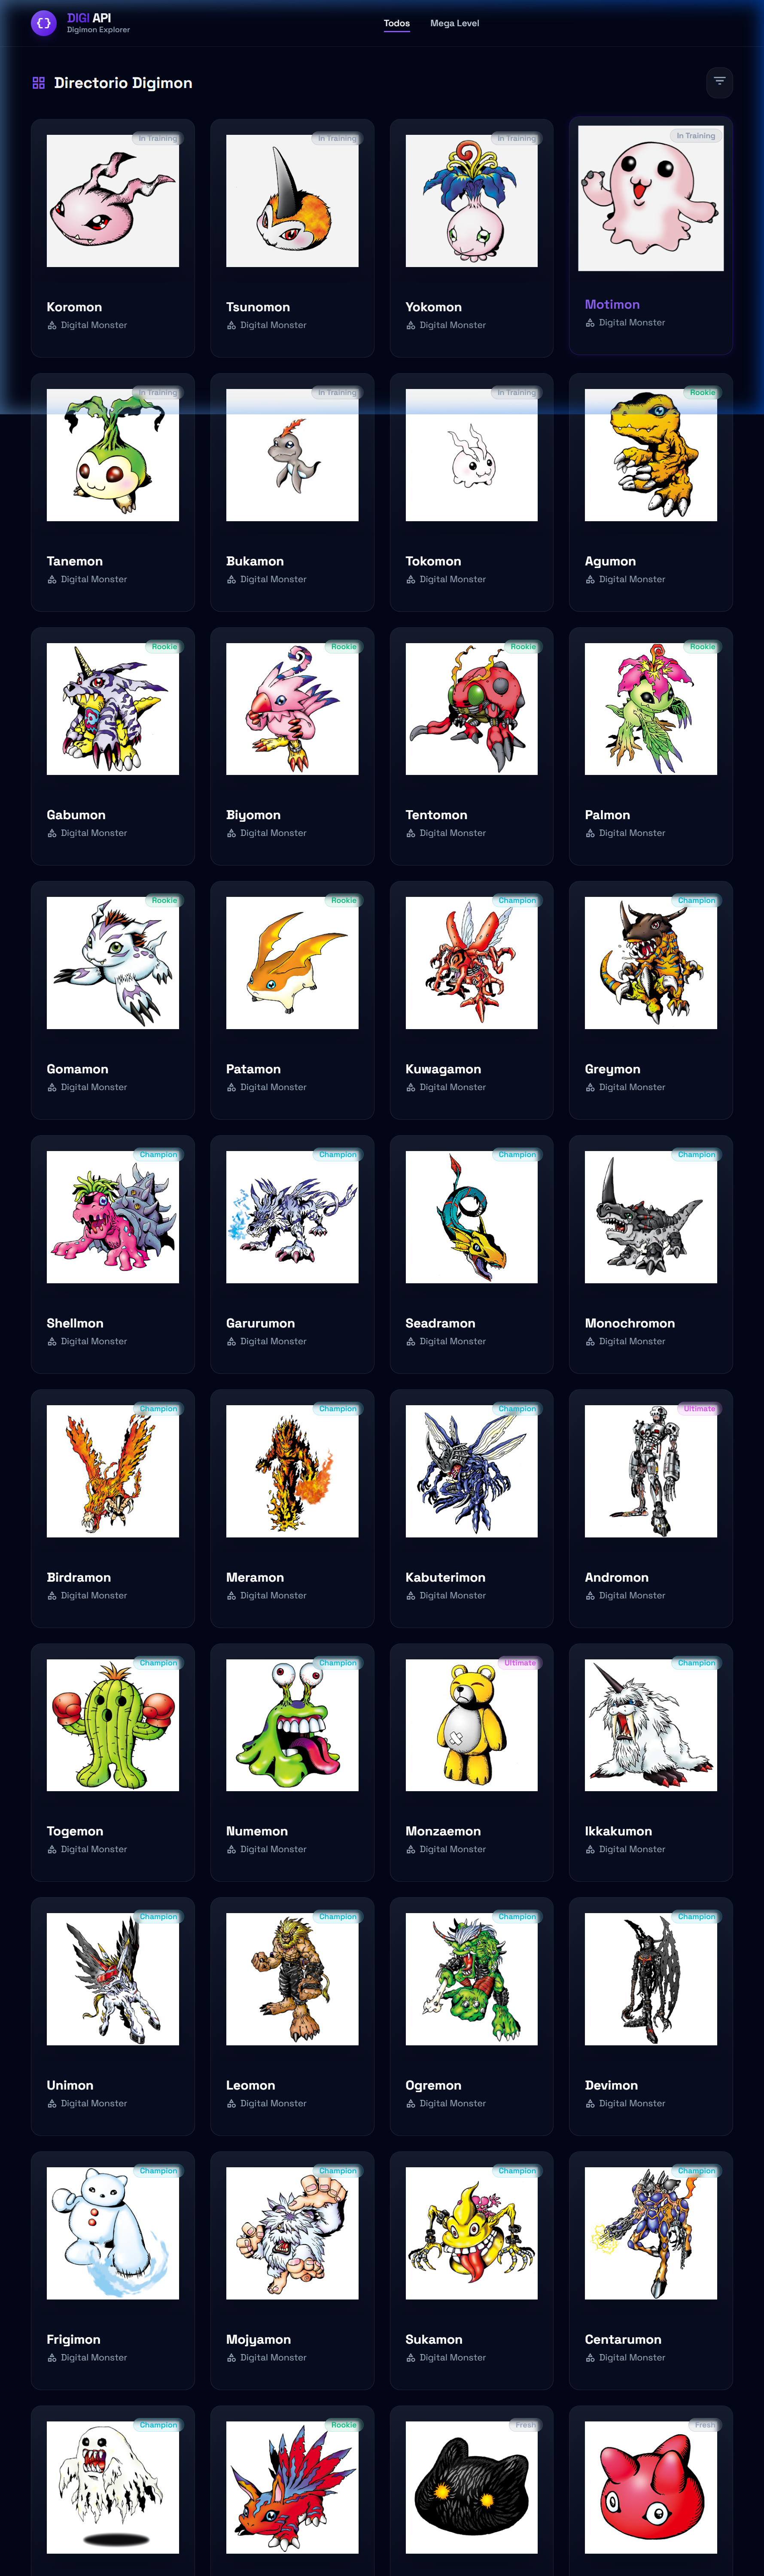
\includegraphics[width=0.4\textwidth]{assets/dashboard.png} \\[2cm]
    
    {\Large \textbf{Luis Emilio Jaras Sánchez}} \\[0.2cm]
    {\large Matrícula: 243697} \\[1.5cm]
    
    {\large \textbf{Docente:}} \\
    {\large Viviana López Rojo} \\[2cm]
    
    {\large \today}
\end{titlepage}

\newpage
\tableofcontents
\newpage

% --- INTRODUCCIÓN ---
\section{Investigación de API Pública}
Para la presente actividad se seleccionó la \textbf{DigiAPI v1}, disponible en \href{https://digimon-api.vercel.app/api/digimon}{digimon-api.vercel.app}. Esta API RESTful proporciona un catálogo extenso de criaturas digitales en formato JSON. Fue elegida por su estructura de datos clara y predecible, permitiendo filtrar por niveles (Rookie, Champion, Mega, etc.) y nombres, lo que facilita la implementación de una interfaz de usuario dinámica, reactiva y con una estética moderna.

% --- ARQUITECTURA ---
\section{Diseño y Arquitectura SOA}
\subsection{Arquitectura Desacoplada (Justificación)}
Se ha implementado una arquitectura basada en \textbf{SOA (Service Oriented Architecture)} estrictamente desacoplada. La separación de responsabilidades, un pilar fundamental de SOA, se divide en tres capas independientes y con responsabilidades únicas:

\begin{itemize}[leftmargin=*]
    \item \textbf{Frontend (Capa de Presentación):} Desarrollada en Next.js y React, está dedicada exclusivamente a la renderización de la interfaz gráfica y a la gestión de la experiencia del usuario (UI/UX). Esta capa es agnóstica a la lógica de negocio; su única responsabilidad es solicitar datos a su backend de confianza y presentarlos de forma atractiva. No conoce la URL de la API de terceros.
    \item \textbf{Backend (Capa de Servicio/Proxy):} Construido con Next.js Route Handlers, actúa como un proxy o mediador entre el cliente y la API externa. Centraliza la lógica de negocio, la seguridad (ocultando la API real), el manejo de CORS y la posible transformación o enriquecimiento de datos. Esta capa protege al sistema de cambios en la API externa.
    \item \textbf{Infraestructura (Capa de Despliegue):} Se utilizan dos instancias independientes de AWS EC2 (t2.micro), una para cada capa (Frontend y Backend), conectadas a través de la red virtual de AWS. Los procesos de Node.js son gestionados por PM2 para garantizar la alta disponibilidad y el reinicio automático ante fallos.
\end{itemize}

\subsection{Diagrama de Arquitectura (TikZ)}
\begin{figure}[h!]
\centering
\begin{tikzpicture}[
    node distance=1.8cm,
    every node/.style={font=\small},
    box/.style={rectangle, draw, thick, minimum width=5.5cm, minimum height=1.7cm, text centered, rounded corners, fill=white},
    arrow/.style={->, thick, >=stealth}
]

% Nodos
\node[box, fill=client!20] (client) {\textbf{Usuario / Navegador}\\ (Cliente HTTP)};
\node[box, fill=frontend!20, below=of client] (frontend) {\textbf{Frontend (Next.js / React)}\\ IP Pública: 3.219.228.71 (Puerto 80)};
\node[box, fill=backend!20, below=of frontend] (backend) {\textbf{Backend Proxy (Next.js API)}\\ IP Pública: 34.225.231.69 (Puerto 3001)};
\node[box, fill=externalapi!20, right=2.5cm of backend] (api) {\textbf{DigiAPI Externa}\\ (digimon-api.vercel.app)};

% Flechas
\draw[arrow] (client) -- node[right, pos=0.4] {Petición a \texttt{http://3.219.228.71}} (frontend);
\draw[arrow] (frontend) -- node[right, pos=0.4] {\texttt{fetch('/api/digimons')}} (backend);
\draw[arrow] (backend.east) -- node[above] {GET Request} (api.west);
\draw[arrow] (api.west) -- ++(-0.5,0) |- node[below, pos=0.8] {Respuesta JSON} (backend.east);
\draw[arrow] (backend) -- node[left, pos=0.6] {Respuesta con CORS} (frontend);
\draw[arrow] (frontend) -- node[left, pos=0.6] {Renderizado de UI} (client);

\end{tikzpicture}
\caption{Diagrama de flujo de datos y arquitectura SOA sobre AWS.}
\end{figure}

\newpage

% --- DESARROLLO Y CONSUMO ---
\section{Desarrollo y Consumo}
\subsection{Peticiones Asíncronas en el Backend}
Para garantizar una arquitectura no bloqueante y eficiente, todas las llamadas desde nuestro Backend Proxy hacia la API externa de Digimon se realizan utilizando el patrón \texttt{async/await} con el cliente HTTP \texttt{axios}.

\begin{lstlisting}[language=TypeScript, caption=Endpoint para obtener todos los Digimons (`/api/digimons/route.ts`)]
import { NextRequest } from 'next/server';
import { digiApiClient } from '@/lib/digiApiClient';
import { jsonResponse, corsMiddleware } from '@/lib/cors';

export async function GET(request: NextRequest) {
    // Aplicar middleware de CORS
    const corsResponse = corsMiddleware(request);
    if (corsResponse) return corsResponse;

    try {
        // Llamada asincrona a la API externa
        const data = await digiApiClient.getDigimons();
        return jsonResponse(data);
    } catch (error: any) {
        return jsonResponse({ error: error.message }, 500);
    }
}
\end{lstlisting}

\subsection{Manejo de Estados de UI en el Frontend}
La aplicación maneja de forma robusta los tres estados de UI requeridos para una experiencia de usuario fluida y profesional:
\begin{enumerate}
    \item \textbf{Loading:} Se utiliza un componente \texttt{LoadingSkeleton} que muestra una cuadrícula de tarjetas animadas con un efecto de pulso. Esto le indica al usuario que la información está en camino y mejora la percepción de velocidad.
    \item \textbf{Success:} Una vez que los datos son recibidos, se renderizan los componentes \texttt{DigimonCard} con la información obtenida. Las tarjetas tienen un diseño "glassmorphism", con efectos de desenfoque y hover para una apariencia premium.
    \item \textbf{Error:} Si la API falla o la red no está disponible, se muestra un componente \texttt{ErrorAlert} con un mensaje amigable, un icono de advertencia y un botón para reintentar la petición.
\end{enumerate}

\section{Enlaces y Repositorios}
\begin{itemize}
    \item \textbf{Aplicación Desplegada (Frontend):} \href{http://3.219.228.71}{\nolinkurl{http://3.219.228.71}}
    \item \textbf{API Desplegada (Backend):} \href{http://34.225.231.69:3001/api/health}{\nolinkurl{http://34.225.231.69:3001/api/health}}
    \item \textbf{Repositorio Frontend en GitHub:} \href{https://github.com/EmilioJaras3/soa-digimon-frontend}{\nolinkurl{github.com/EmilioJaras3/soa-digimon-frontend}}
    \item \textbf{Repositorio Backend en GitHub:} \href{https://github.com/EmilioJaras3/backend--digi-api}{\nolinkurl{github.com/EmilioJaras3/backend--digi-api}}
\end{itemize}


\newpage

% --- CAPTURAS ---
\section{Evidencias del Proyecto}

\subsection{Dashboard Principal en AWS}
\begin{figure}[h!]
    \centering
    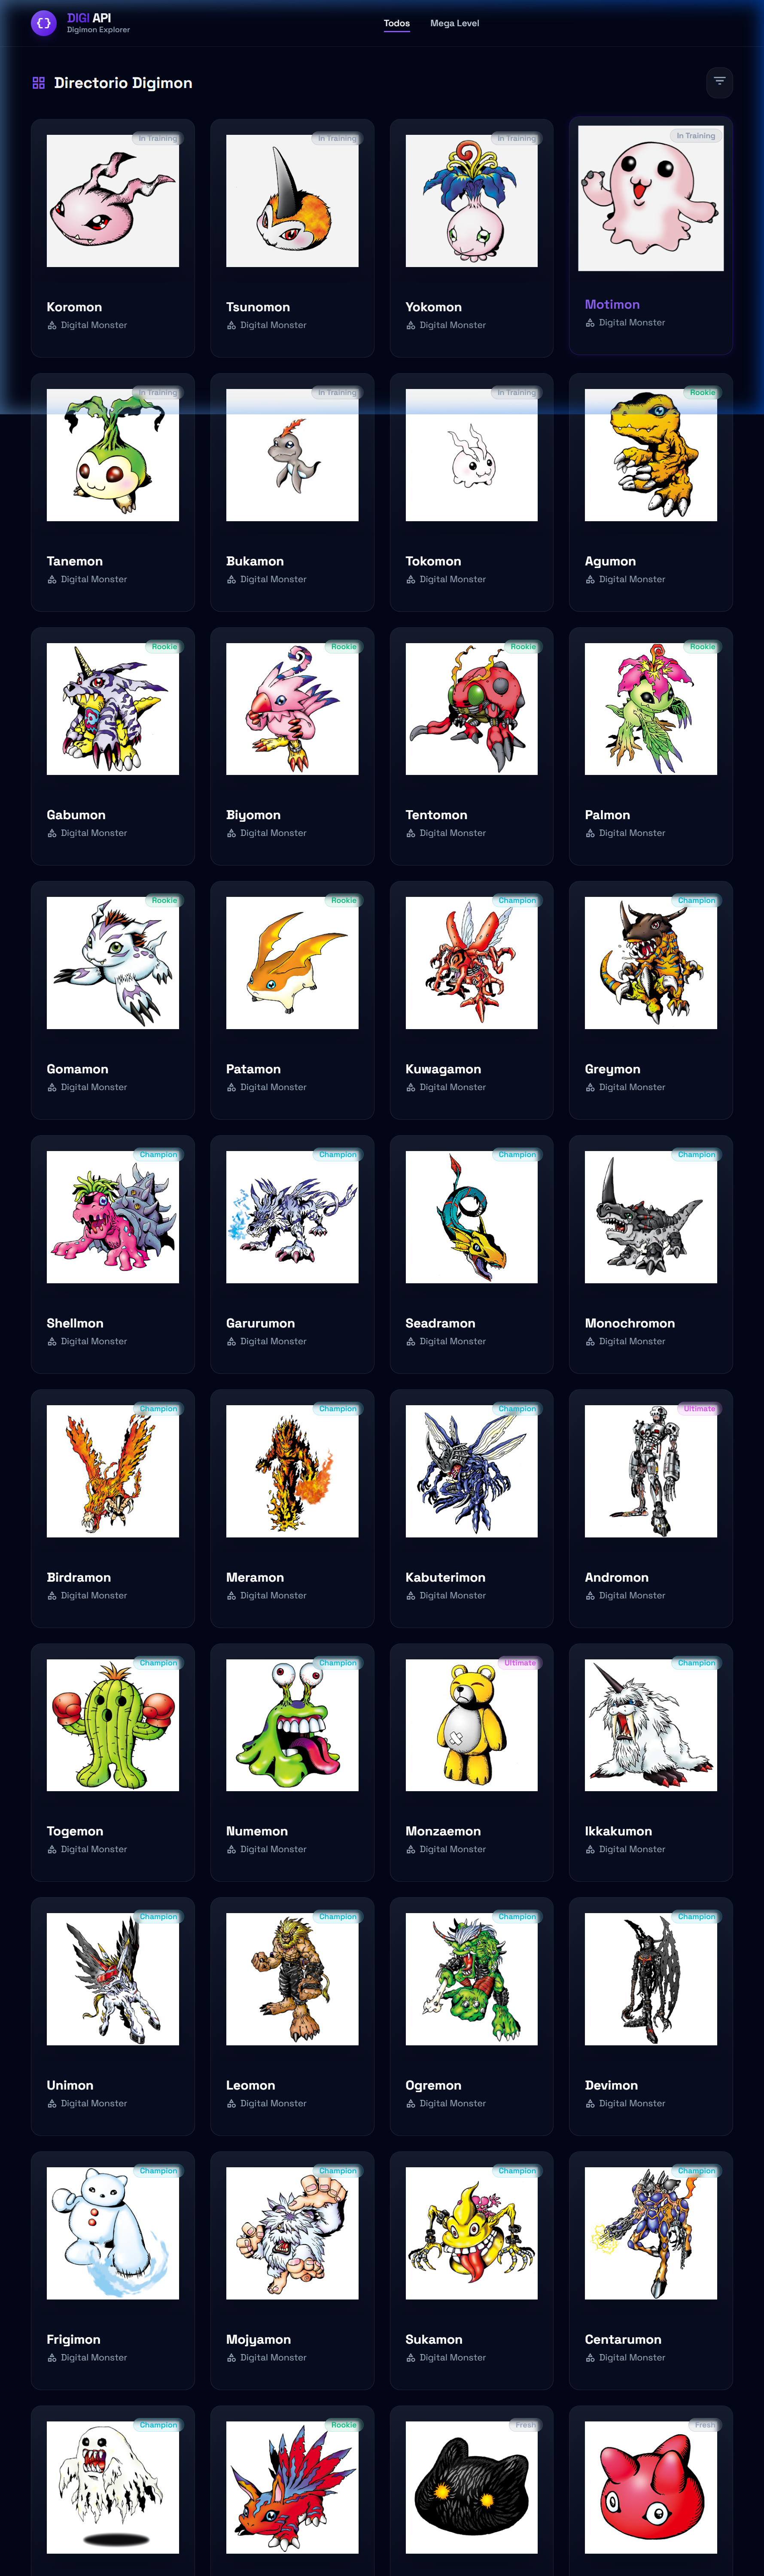
\includegraphics[width=\textwidth]{assets/dashboard.png}
    \caption{Dashboard de Digimon Explorer funcionando sobre la IP pública de la instancia EC2 de frontend.}
\end{figure}

\subsection{Filtro por Nivel "Mega"}
\begin{figure}[h!]
    \centering
    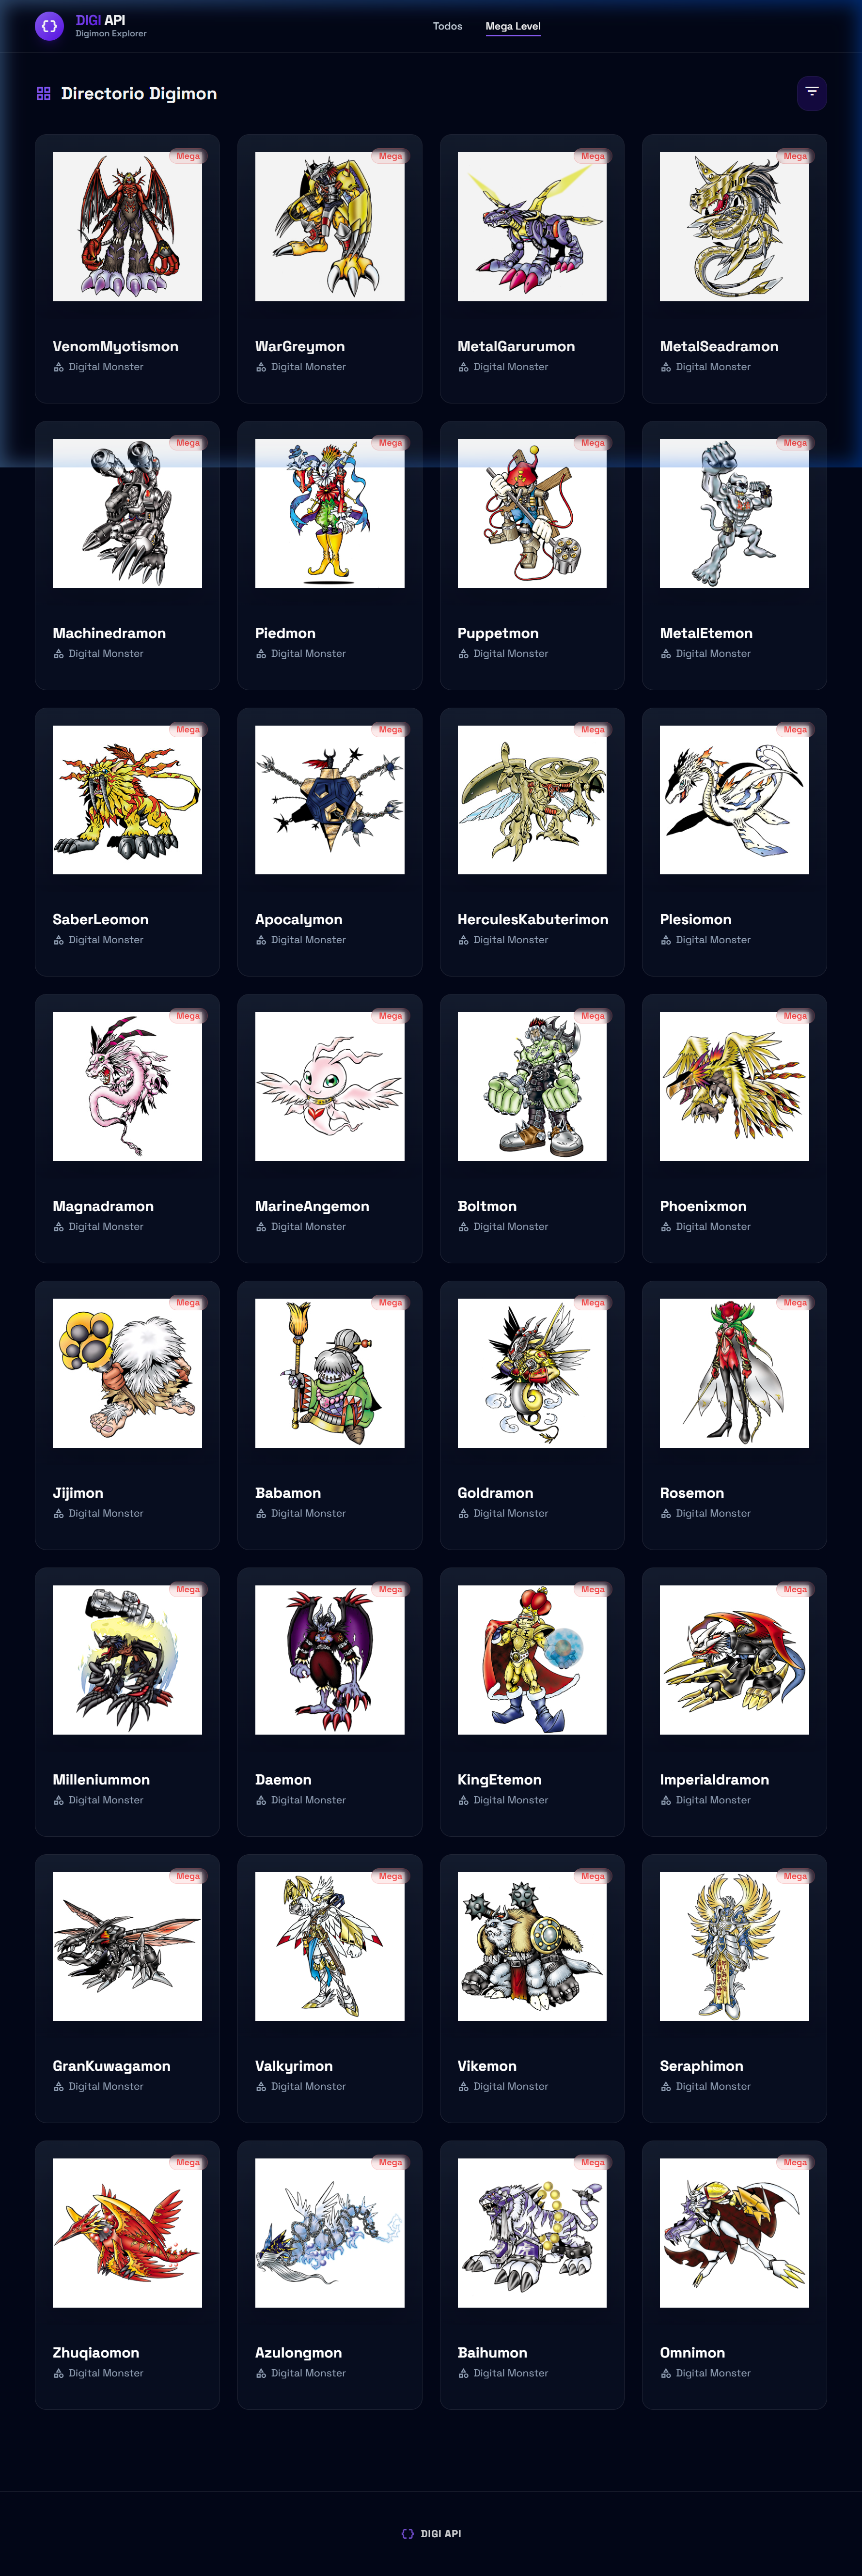
\includegraphics[width=\textwidth]{assets/filters.png}
    \caption{La interfaz reacciona al filtro "Mega", solicitando y renderizando únicamente los Digimons de ese nivel desde el endpoint \texttt{/api/mega}.}
\end{figure}

\newpage
\subsection{Endpoint de Salud del Servicio}
\begin{figure}[h!]
    \centering
    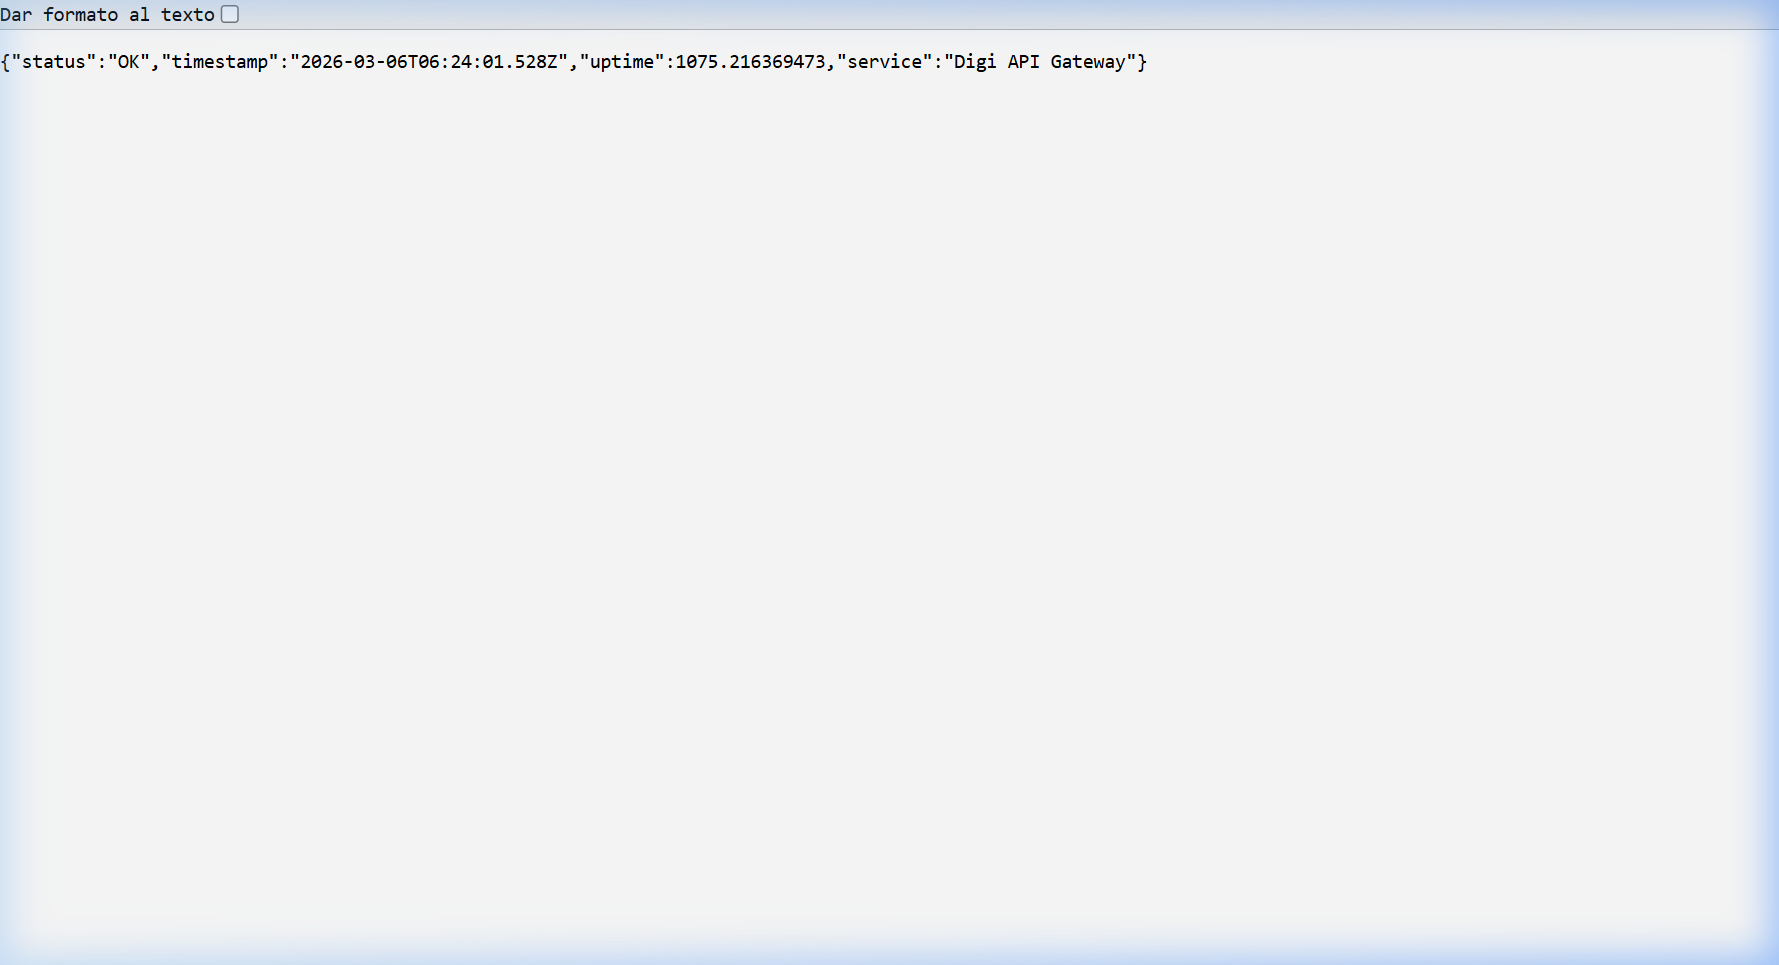
\includegraphics[width=0.9\textwidth]{assets/health.png}
    \caption{Respuesta JSON del endpoint \texttt{/api/health}, que indica el estado del servicio y su tiempo de actividad (uptime) en segundos.}
\end{figure}

\section{Configuración de Infraestructura en AWS}
\subsection{Aislamiento y Redirección de Puertos}
Se configuró una regla en el \textbf{Security Group} de la instancia frontend para permitir tráfico HTTP entrante en el puerto 80. Para evitar que los usuarios necesiten escribir el puerto de la aplicación (3002), se utilizó \texttt{iptables} en el servidor Ubuntu para redirigir todo el tráfico del puerto 80 al 3002.
\begin{lstlisting}[language=bash]
sudo iptables -t nat -A PREROUTING -p tcp --dport 80 -j REDIRECT --to-port 3002
\end{lstlisting}

\subsection{Gestión de Procesos con PM2}
Los procesos de Node.js en ambas instancias son administrados por PM2. Esto asegura que las aplicaciones se reinicien automáticamente si fallan y facilita la gestión de logs y el monitoreo de recursos.
\begin{lstlisting}[language=bash, caption=Estado del proceso frontend en AWS vía PM2]
┌────┬─────────────────┬───────────┬──────┬─────────┬──────────┬────────┬───┬──────────┬───────┬──────────┐
│ id │ name            │ namespace │ mode │ pid     │ uptime   │ ↺  │ status │ cpu   │ mem   │ user   │
├────┼─────────────────┼───────────┼──────┼─────────┼──────────┼────────┼───┼──────────┼───────┼──────────┤
│ 0  │ digi-frontend   │ default   │ fork │ 19747   │ 4m       │ 8  │ online │ 0%    │ 55mb  │ ubuntu │
└────┴─────────────────┴───────────┴──────┴─────────┴──────────┴────────┴───┴──────────┴───────┴──────────┘
\end{lstlisting}

\section{Conclusiones}
La implementación de una arquitectura SOA para el consumo de la DigiAPI demostró ser una estrategia robusta y escalable. Al utilizar una capa intermedia (Backend Proxy), se resolvieron problemas críticos de seguridad como el \textbf{CORS} y se abstrajo la complejidad de la API de terceros del cliente final. El desacoplamiento estricto entre el frontend y el backend no solo es una buena práctica, sino que facilita el mantenimiento y la evolución independiente de cada capa.

El despliegue en la nube sobre AWS EC2 con gestión de procesos mediante PM2 proporcionó un entorno de producción realista, garantizando que la aplicación sea accesible, resiliente y con un rendimiento adecuado para una experiencia de usuario profesional. Este proyecto ha sido un ejercicio práctico integral que abarca desde el diseño arquitectónico hasta el despliegue final en la nube.

\section{Fuentes de Consulta}
\begin{itemize}[leftmargin=*]
    \item DigiAPI v1 Documentation: \url{https://digimon-api.vercel.app/}
    \item Next.js Official Docs (App Router \& Route Handlers): \url{https://nextjs.org/docs}
    \item Amazon Web Services (AWS EC2 Documentation): \url{https://aws.amazon.com/ec2/}
    \item PM2 - Advanced Node.js Process Manager: \url{https://pm2.keymetrics.io/}
    \item MDN Web Docs (Cross-Origin Resource Sharing - CORS): \url{https://developer.mozilla.org/en-US/docs/Web/HTTP/CORS}
\end{itemize}

\end{document}
